\documentclass{amsart}

\usepackage{graphicx}
\usepackage{caption}
\usepackage{subcaption}

\newtheorem{theorem}{Theorem}[section]
\newtheorem{lemma}[theorem]{Lemma}

\theoremstyle{definition}
\newtheorem{definition}[theorem]{Definition}
\newtheorem{example}[theorem]{Example}
\newtheorem{xca}[theorem]{Exercise}

\theoremstyle{remark}
\newtheorem{remark}[theorem]{Remark}

\numberwithin{equation}{section}

%    Absolute value notation
\newcommand{\abs}[1]{\lvert#1\rvert}

%    Blank box placeholder for figures (to avoid requiring any
%    particular graphics capabilities for printing this document).
\newcommand{\blankbox}[2]{%
  \parbox{\columnwidth}{\centering
%    Set fboxsep to 0 so that the actual size of the box will match the
%    given measurements more closely.
    \setlength{\fboxsep}{0pt}%
    \fbox{\raisebox{0pt}[#2]{\hspace{#1}}}%
  }%
}

\begin{document}

\title{A Proposed Neural Network Activation Function}

\author{Matthew Schroeder}

\date{March 11, 2019}

\begin{abstract}
In this paper a new activation function for deep neural networks is presented.  Their are two variants of the activation function. The first is a smooth, oscillatory version of ReLU. The second is a smooth, oscillatory version of ReLU with exponential decay of the oscillations.
\end{abstract}

\maketitle

\section{INTRODUCTION}
The primary reason neural networks are so successful at solving problems in machine learning is their ability to create highly non-linear functions.   The feature of a neural network which makes this possible is the activation function.  The activation function takes what is otherwise a linear object and makes it non-linear.  It is no surprise then, that discovering new activation functions to use in neural networks is an ongoing area of research.   

The most popular activation function used today is the rectified linear unit (ReLU).  The most attractive property of ReLU seems to be its simplicity; the computation of this function and its derivative is very fast, which simplifies and accelerates the training of neural networks. ReLU, however, is not differentiable at the origin, which has lead to the search for other activation function which are differentiable at the origin and have similar properties.  The purpose of this paper is to present two such activation functions.    

The function which is the basis for the activation functions I will discuss is $$f(x) = \min(1, \max(0, x - \frac{1}{2\pi}\sin(2\pi x)))$$ In the past I have used this function to ramp a servo hydraulic actuator between points. It was chosen since it has continuous first and second derivatives and discontinuities in velocity or acceleration can damage some kinds of specimens (discontinuity in the jerk is tolerated).  A glance at the graph (fig. 1) reveals that this is a Sigmoid function and so, naturally, activation functions came to mind.   

\begin{figure}[tb]
%\blankbox{.75\columnwidth}{3pc}
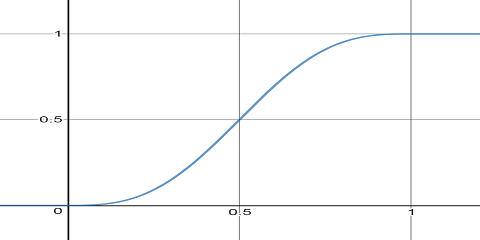
\includegraphics[1]{xsinx.png}
\caption{The graph of $f(x) = \min(1, \max(0, x - \frac{1}{2\pi}\sin(2\pi x)))$}
\label{Figure 1}
\end{figure}  

The goal of this paper is not to look at $x-\sin(x)$ as a replacement for the logistic function, but instead is to use $x-\sin(x)$ to create smooth versions of ReLU.   The two activation functions I will consider are shown in the Table 1 (simplest form).  The first is called Oscillating ReLU (OscReLU) )and the second Oscillating ReLU with Exponential Decay (DOscReLU). Both resolve the issue of non-differentiability at zero. 

\begin{table}[!h]
\renewcommand\arraystretch{1.5}
\noindent\[
\begin{array}{|c|c|}
\hline
OscReLU & \max(0, x - \frac{1}{2\pi}\sin(2\pi x)\\
\hline
DOscReLU & \max(0, x - \frac{1}{2\pi}e^{-sx^2}\sin(2\pi x)\\
\hline
\end{array}
\]
\end{table}

This paper is organized as follows. In section 2 ReLU will be discussed. In section 3 the new activation functions are discussed. Section 4 contains an analysis of experimental results.  Finally a conclusion is given in section 5.  

\section{ReLU}  

ReLU was introduced as a replacement for the logistic function and tanh. The formulas for ReLU and its derivative are given by $$f(x) = max(0, x)$$ $$f'(x) = \begin{cases}0 : x < 0 \\ 1 : x \geq 0 \end{cases}$$ The graph of ReLU and of its derivative are shown in Figure 2.  

\begin{figure}[!h]
%\blankbox{.75\columnwidth}{3pc}
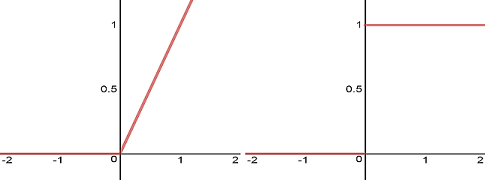
\includegraphics[1]{ReLU.png}
\caption{ReLU and its derivative}
\label{Figure 2}
\end{figure}  

The Logistic function and tanh both have bounded range and have derivatives which asymptotically approach zero (very quickly).  This leads to a phenomena known as the Vanishing Gradient Problem.  Essentially as the gradient goes to zero at a given neuron, it will now longer contribute during back propagation. ReLU solves this problem, at least for positive inputs.  

ReLU is very simple, its use in the network, involves just a comparison, addition and multiplication.  In addition the derivative of ReLU is just a step function. These properties are to be compared with the rather complex formulas and derivative for other activation functions.  The computational simplicity and efficiency of ReLU, coupled with the fact that it works are the reasons it is so popular.   

In addition to ReLU, I will be comparing the performance of OscReLU and DOscReLU to two recent state of the art activation functions: Swish \cite{A} and LiSHT \cite{B}. The formulas and graphs of these functions are shown below.   

Swish  $f(x) = x \dot \sigmoid(βx)$ \hfill\break
LiSHT  $f(x) = x \dot \tanh(x)$

\begin{figure}[!h]
%\blankbox{.75\columnwidth}{3pc}
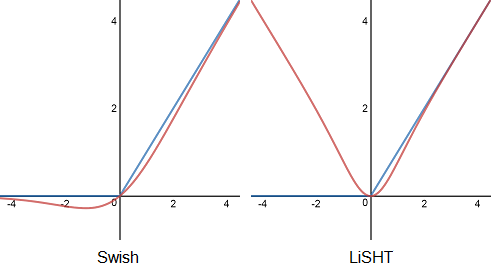
\includegraphics[1]{swish_with_LiSHT.png}
\caption{Swish and LiSHT. ReLU is plotted as well for reference}
\label{Figure 3}
\end{figure}  

\hfill\break
\section{OscReLU and DOscReLU}  

The goal of these two activation functions is to introduce a higher level of non-linearity than ReLU, while attempting to maintain many of the favorable properties. The most general formulas for OscReLU and DOscReLU includes parameters. 
The following functions have parameters S,I, and K, which are define as:  S is a horizontal shift which allows the dying gradient of the function to be shifted into the negative half plane, I is a vertical shift, called the inhibitory offset (to be explained below), and, finally, K is the decay rate of the exponential.  
\newpage
\subsection{OscReLU}  \hfill \break 
\hfill\break
$f(x,S,I) = \max(0, (x + S) - \frac{1}{2\pi}\sin(2\pi (x+S)) - I$ \hfill \break
\hfill\break
$f'(x,S,I) = \begin{cases} 1 - cos(2\pi (x+S)) & x \geq -S \\ 0 & x < -S\end{cases}$ \hfill \break

\begin{figure}[!h]
%\blankbox{.75\columnwidth}{3pc}
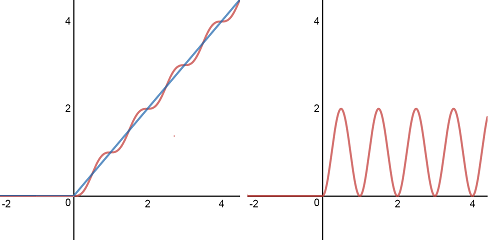
\includegraphics[1]{OscReLU_with_ReLU_Derive.png}
\caption{OscReLU and its derivative with S = 0 and I = 0}
\label{Figure 4}
\end{figure}  

In Figure 4, ReLU is shown on the plot of OscReLU for comparison. As can be seen OscReLU oscillates around ReLU with flat inflection points at the integers. This is a simple with a simple derivative, like ReLU. The version shown here has both parameters set to 0, this is not the best configuration.  Also notice that this will give a sparse network like ReLU.   

\subsection{DOscReLU}  \hfill \break 
\hfill\break
$f(x,S,I,K) = \max(0, (x + S) - \frac{1}{2\pi}e^{-K(x+S)^2}\sin(2\pi (x+S)) - I$ \hfill \break 
\hfill\break
$f'(x,S,I,K) = \begin{cases}\frac{1.0}{\pi}(x+S)e^{-K(x+S)^2}\sin(2\pi(x+S))-e^{-K(x+S)^2}\cos(2\pi(x+S)) + 1 & x \geq -S \\ 0 & x < -S \end{cases}$ \hfill \break 

\begin{figure}[!h]
%\blankbox{.75\columnwidth}{3pc}
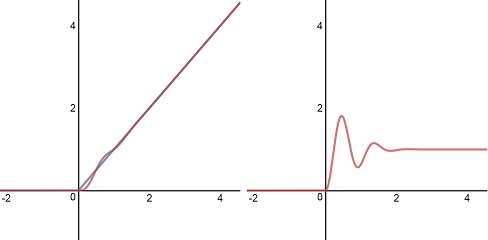
\includegraphics[1]{DOscReLU_with_ReLU_Deriv.png}
\caption{DOscReLU and its derivative with S = 0, I = 0, and K = 1}
\label{Figure 5}
\end{figure}  

This is not a simple function and its derivative is not simple.  It is very similar to OscReLU except the oscillations around the ReLU decay to zero exponentially.   
Now to discuss the parameters for these functions.  

\newpage
\subsubsection{Decay Rate K} \hfill\break  

This parameter only applies to DOscReLU and controls the rate at which the oscillations of the curve around ReLU decays.  Figure 6 shows the oscillations for three values of K.  During tests I left the decay rate at 1.0.

\begin{figure}[!h]
%\blankbox{.75\columnwidth}{3pc}
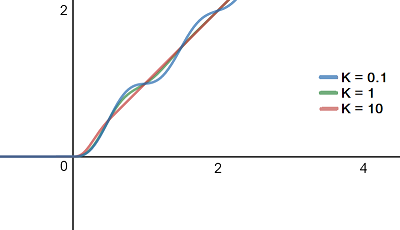
\includegraphics[1]{DecayRate.png}
\caption{Parameter K for DOscReLU}
\label{Figure 6}
\end{figure} 

\subsubsection{Horizontal Shift S} \hfill\break  

\begin{figure}[!h]
%\blankbox{.75\columnwidth}{3pc}
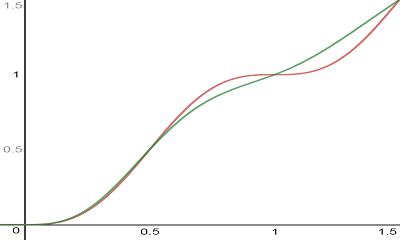
\includegraphics[1]{Shift.png}
\caption{Parameter S near zero}
\label{Figure 7}
\end{figure} 

Consider Figure 7. We see that as x approaches zero from the right, the gradient goes to zero.  It is undesirable to have the gradient go to zero near the origin in the positive half plane. S can be used to shift the curve left so the gradient vanishes in the negative half plane.  I averaged the test accuracy of 10 trials of 15 training iterations of the network for each of 10 shift values in order to determine the best left shift.  Figure 8 shows the results.  I determined that 
S = 0.75 for OscReLU and S = 1 for DOscReLU performed well.  The resulting activation functions are shown in Figure 9.

\begin{figure}[!h]
%\blankbox{.75\columnwidth}{3pc}
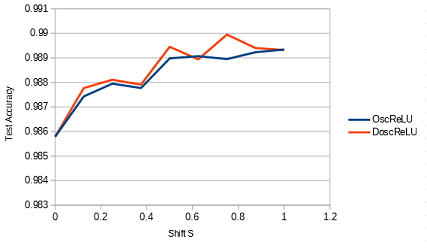
\includegraphics[1]{ShiftTest.png}
\caption{Test Accuracy vs. Shift Left}
\label{Figure 8}
\end{figure} 

\begin{figure}[!h]
%\blankbox{.75\columnwidth}{3pc}
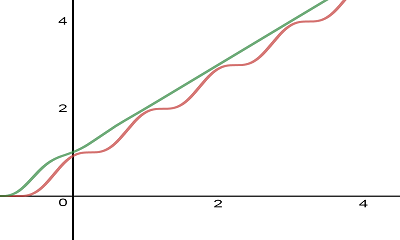
\includegraphics[1]{ShiftedCurves.png}
\caption{Shifted Activation Functions}
\label{Figure 9}
\end{figure} 

\subsubsection{Inhibitory Offset I} \hfill\break   

It seems that one should be careful about making biological analogies to motivate neural network design. Given that, I am going to make some biological analogies to motivate the inhibitory offset parameter.  ReLU was first introduced by Hahnloser et. al, 2000 \cite{C}.  In this paper ReLU was given biological motivations.  The zero output on the negative axis was supposed to correspond to the threshold of the action potential (negative inputs do not pass the threshold).  The unbounded slope is supposed to represent the property that connections between neurons are strengthened with increasing frequency of firing of the presynaptic neuron (the high frequency trains of action potentials cause increased density of neurotransmitter receptors on the postsynaptic neuron).  I am dubious about both of these interpretations.  There are inhibitory as well as excitatory synapses.  An example is the Neurotransmitter GABA, which plays a major role in inhibitory action in the retina.  GABA receptors cause $\text{CL}^-$ ion channels to open.  This influx of negative ions counteracts the influx of $\text{NA}^+$ and $\text{K}^+$ generated by excitatory neurotransmitters.  It seems unusual (and this may be my naivete about neural networks) to set all negative inputs to output zero.  Note that both Swish and LiSHT introduce non-zero outputs on the negative axis.  Both of these activation functions have been shown to outperform  ReLU.  I am not sure if simply allow for output on the negative axis is a good model of inhibitory synapses.  Finding a way to model inhibitory effects seems like an interesting problems.  I have introduced the parameter I to allow the curves to be shifted down and therefore allow the forwarding of negative values.  If this has not convinced the reader, then consider this.  The prefrontal cortex is known to contain neurons which act to inhibit the limbic system.  Individuals with a damaged or malfunctioning prefrontal cortex have impulse control and often engage in criminal activity including violence. fMRI scans of psychopaths have shown abnormalities and diminished activity in the cingulate cortex, a part of the prefrontal cortex.  This lack of proper signalling from the frontal cortex to the limbic through the prefrontal cortex is explanatory of the condition.  So, unless you want you neural network to act like a psychopath, it may be a good idea to introduce inhibitory action.  (I apologize for that).  I will train a couple models with I set to 0.5 and see what happens.  The two activation functions will be OscReLU(0.5,0.5) and DOscReLU(1.0,0.5,1.0). These are pictured in Figure 10.  
\begin{figure}[!h]
%\blankbox{.75\columnwidth}{3pc}
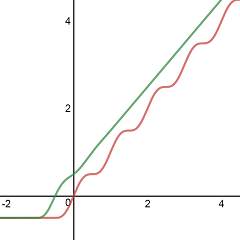
\includegraphics[1]{Inhib.png}
\caption{OscReLU(0.5,0.5) and DOscReLU(1.0,0.5,1.0)}
\label{Figure 10}
\end{figure} 

\section{Test Results}   

To do initial testing of these activation functions, I choose a very simple neural network.  I found the code for this network online in an article called  "Image Classification in 10 Minutes with MNIST Dataset" \cite{D}. As you can tell by the name this is an elementary network. It is a 5 layer CNN. I ran each activation through this network 10 times for 15 iterations each.  I averaged the results to get the test performance.  The following table shows the results.  

\begin{table}[!h]
\renewcommand\arraystretch{1.5}
\noindent\[
\begin{array}{|c|c|c|}
\hline
 & Test Accuracy & Standard Error\\
\hline
ReLU & 0.9854 & 0.0011\\
\hline
OscReLU(0.5,0) & 0.9890 &  0.0010\\
\hline
DOscReLU(1,0,1) & 0.9893 & 0.0005\\
\hline
Swish & 0.9855 & 0.0007\\
\hline 
LiSTH & 0.9869 & 0.0009 \\
\hline
OscReLU(0.5,0.5) & 0.9885 & 0.0015 \\
\hline
\end{array}
\]
\end{table}

OscReLU and DOscReLU slightly outperform the three other activation functions for this neural network. 
\section{Conclusion}  

These activation functions show some promise. On this small neural network they performed quite well.  My next step is to test on deeper networks and on different kinds of networks with different data sets.

\bibliographystyle{amsplain}
\begin{thebibliography}{10}

\bibitem {A} S.K. Roy, S. Manna, S.R. Dubey, B. Chaudhuri, \textit{LiSHT: Non-Parametric Linearly Scaled Hyperbolic Tangent Activation Function for Neural Networks} ArXIV:1901.05894v1 (2019)

\bibitem {B} P. Ramachandran, B. Zoph, Q.V. Le, \textit{SEARCHING FOR ACTIVATION FUNCTIONS}, ArXIV:1710.05894v1 (2019)

\bibitem {C} R. Hahnloser et al, \textit{Digital selection and analogue amplification coexist in a cortex-inspired silicon circuit}, ArXIV:1710.05894v1 (2019)

\bibitem {D} O. Yalchin, “Image Classification in 10 Minutes with MNIST Dataset.” Towards Data Science, Towards Data Science, 19 Aug. 2018, towardsdatascience.com/image-classification-in-10-minutes-with-mnist-dataset-54c35b77a38d

\end{thebibliography}

\end{document}

%------------------------------------------------------------------------------
% End of journal.tex
%------------------------------------------------------------------------------
